\chapter{画图 tikz}

\section{使用代码嵌入还是文件嵌入}

在 \LaTeX 中使用 TikZ 绘图有两种主要方式:直接嵌入代码和外部生成后嵌入。两种方法各有优缺点。

\subsection{比较}

先说结论:两种方式都能保留矢量效果;外部生成后嵌入的方式编译速度明显更快。

实践建议:简单图形 - 直接嵌入LaTeX文档;复杂图形 - 使用externalize功能;超复杂图形 - 考虑完全外部化,使用单独的文件生成后导入;需要频繁修改调试的图形 - 先在单独文件中开发和测试,完成后再整合到文档中。

\subsubsection{直接嵌入TikZ代码}

\paragraph{优点}

\begin{itemize}
    \item 保留完整矢量图质量,缩放不失真
    \item 图形字体与文档保持一致性
    \item 便于随时修改图形
    \item 可引用文档中的变量和参数
    \item 与文档完全集成,便于版本控制
\end{itemize}

\paragraph{缺点}

\begin{itemize}
    \item 编译速度较慢,每次都需重新生成图形
    \item 复杂图形会消耗大量内存
    \item 调试可能较为困难
\end{itemize}

\subsubsection{外部生成PDF后嵌入}

\paragraph{优点}

\begin{itemize}
    \item 编译速度快,图形只需生成一次
    \item 降低主文档复杂度
    \item 图形可在多个文档中重用
    \item 可单独调试图形
\end{itemize}

\paragraph{缺点}

\begin{itemize}
    \item 工作流程较复杂,需维护额外文件
    \item 修改图形需重新编译外部文件
    \item 无法直接引用主文档中的变量
\end{itemize}

\subsection{最佳实践:TikZ外部化功能}

可使用 \mintinline{latex}{externalize} 库结合两种方法的优点:

\begin{listing}[H]
    \begin{minted}{latex}
        \usepackage{tikz}
        \usetikzlibrary{external}
        \tikzexternalize[prefix=tikz/]
    \end{minted}
    \caption{导言区external宏包以及配置}
    \lablistings{导言区external宏包以及配置}
\end{listing}

\begin{figure}[htbp]
    \centering
    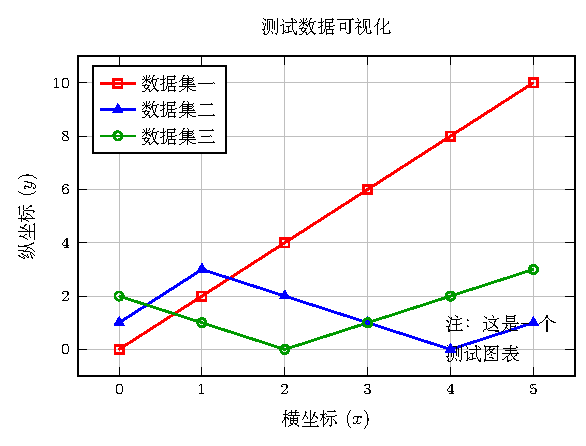
\includegraphics[width=0.6\textwidth]{plots/plot_test.pdf}
    \caption{这是一个通过独立编译生成的测试数据可视化图表。}
    %\label{fig:my_plot} % 为图表设置一个标签,方便交叉引用
\end{figure}